\section{Research Objective 2: Develop data-parallel methods for evaluating Boolean circuits}
\begin{frame}
    \Large{\centerline{\textbf{Research Objective 2}}}
    \vspace{6pt}
    \large{\centerline{\textbf{Develop data-parallel methods for evaluating Boolean circuits}}}
\end{frame}

%% ------------------------------------------------------------------
%% From Truth Table to Bit-Parallelism
%% ------------------------------------------------------------------
\subsection{Bitwise Kernels}
\begin{frame}{Boolean Truth Table – Single Bit}
\centering
\begin{tabular}{c|c|c|c|c|c|c|c}
$X$ & $Y$ & AND & OR & XOR & NAND & NOR & XNOR \\ \hline
0 & 0 & 0 & 0 & 0 & 1 & 1 & 1 \\
0 & 1 & 0 & 1 & 1 & 1 & 0 & 0 \\
1 & 0 & 0 & 1 & 1 & 1 & 0 & 0 \\
1 & 1 & 1 & 1 & 0 & 0 & 0 & 1 \\
\end{tabular}
\vspace{8pt}
\begin{itemize}
  \item Classical gate evaluation operates \emph{bit-by-bit}.  Throughput $\propto$ number of Boolean operations.
  \item Perform \textbf{64} of these truth-table lookups in one machine instruction.
\end{itemize}
\end{frame}

%% ------------------------------------------------------------------
%% Eight Bits in Parallel
%% ------------------------------------------------------------------
\begin{frame}{Extending to a 64-Bit Word}
\begin{columns}
  \column{0.55\textwidth}
    \begin{itemize}
      \item Pack 64 independent Bernoulli trials into one byte.
      \item Bitwise primitives act \emph{independently} on every bit position.
      \item Hardware native instructions guarantee ns latency.
    \end{itemize}
  \column{0.45\textwidth}
    \centering
    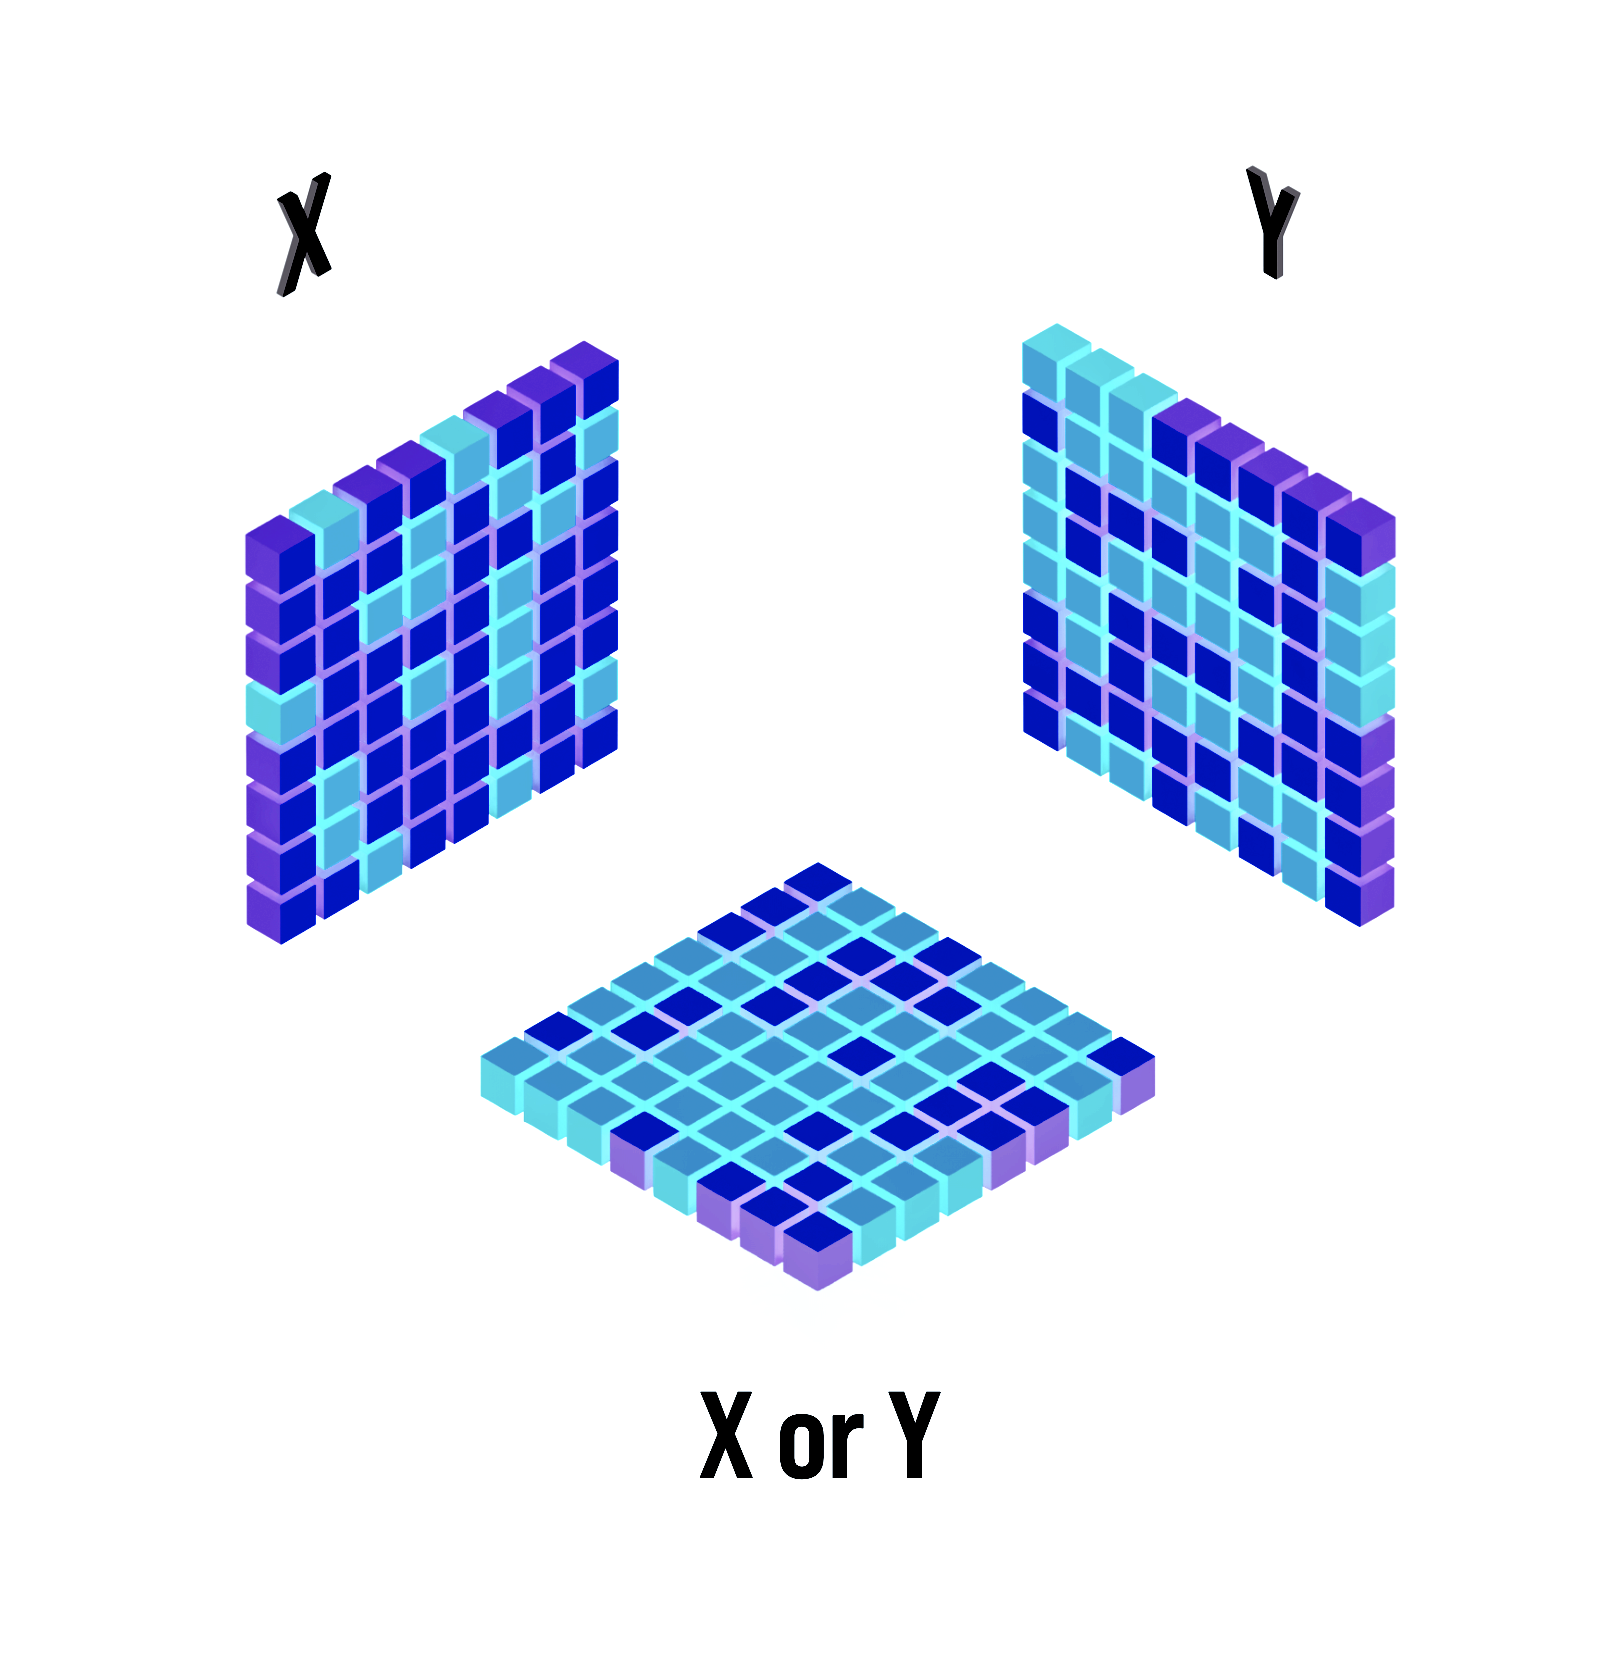
\includegraphics[height=0.7\textheight]{2_framework/research_objective_2_sycl_eval/bitwise_xy_inv.png}
\end{columns}
\end{frame}


% special case for k/n kernels
% ------------ Slide 1a : Original Voting Gate -----------------
\begin{frame}[t]{What is a $k$-of-$n$ (Voting) Gate?}
  \begin{columns}
    % Gate graphic
    \column{0.30\textwidth}
      \centering
    \begin{figure}[h!]
    \tikzset{
    grow'=down,
    level distance=16pt,
    % sibling distance=24pt,
    % sibling distance=8mm/#1,
    level/.style={sibling distance=3pt+44pt/(#1*#1*0.75)},
    edge from parent/.append style={
        draw,
        %thick,
        edge from parent path={
        (\tikzparentnode.west) |- ($(\tikzparentnode.west)!0.5!(\tikzchildnode.east)$) -| (\tikzchildnode.east)
        },
    },
    every node/.append style={
        anchor=center,
        rotate=90,
        draw=black,
        fill=white,
        thick,
        font=\footnotesize\bfseries,
        text centered,
        inner sep=0pt
    },
    var/.style={
        shape=circle,
        minimum height=16pt,
    },
    and/.style={
    and gate US,
    },
  not/.style={
    not gate US,
  },  
  or/.style={
    or gate US,
  },
  vot/.style={
    or gate US,
  }
}
    \centering
    \resizebox{\textwidth}{!}{%
\begin{tikzpicture}[
    circuit logic US,
    tiny circuit symbols,
    level 1/.style={sibling distance=18pt},
    level 2/.style={sibling distance=18pt},
    ]
  \node[or]{\rotatebox{-90}{\tiny{3/5}}}
  % Subset of size 5
  child {
    child { node[var] {\rotatebox{-90}{$X_1$}} }
    child { node[var] {\rotatebox{-90}{$X_2$}} }
    child { node[var] {\rotatebox{-90}{$X_3$}} }
    child { node[var] {\rotatebox{-90}{$X_4$}} }
    child { node[var] {\rotatebox{-90}{$X_5$}} }
  };
\end{tikzpicture}
    }
    \label{fig:example-3of5-voter-tree_no_expansion}
\end{figure}

      \\[-4pt] \scriptsize Example: $k=3$, $n=5$
    % Bullets
    \column{0.70\textwidth}
      \begin{itemize}[<+->]
        \item Outputs 1 iff at least $k$ of $n$ inputs are 1 (majority / threshold logic).
        \item Classic PRA models expand this gate into basic AND/OR primitives --> leads to combinatorial blow-up.
      \end{itemize}
  \end{columns}
\end{frame}

% ------------ Slide 1b : Naïve AND/OR Expansion -----------------
\begin{frame}[t]{Naïve Expansion => Combinatorial Explosion}
  \begin{columns}
    % Left: bullet explanation
    \column{0.35\textwidth}
      \begin{itemize}[<+->]
        \item Expansion = OR of every subset with $k,\dots,n$ true inputs.
        \item For $n=5$, $k=3$: $\binom{5}{3}=10$ conjunction clauses => 26 total gates after binary-tree lowering.
        \item Complexity becomes $\Theta(2^{n}/\sqrt{n})$ at $k\approx n/2$.
      \end{itemize}
    % Right: expanded tree graphic
    \column{0.65\textwidth}
      \centering
      \begin{figure}[h!]
    \tikzset{
    grow'=down,
    level distance=42pt,
    % sibling distance=24pt,
    % sibling distance=8mm/#1,
    level/.style={sibling distance=3pt+44pt/(#1*#1*0.75)},
    edge from parent/.append style={
        draw,
        %thick,
        edge from parent path={
        (\tikzparentnode.west) |- ($(\tikzparentnode.west)!0.5!(\tikzchildnode.east)$) -| (\tikzchildnode.east)
        },
    },
    every node/.append style={
        anchor=center,
        rotate=90,
        draw=black,
        fill=white,
        thick,
        font=\footnotesize\bfseries,
        text centered,
        inner sep=0pt
    },
    var/.style={
        shape=circle,
        minimum height=16pt,
    },
    and/.style={
    and gate US,
    },
  not/.style={
    not gate US,
  },  
  or/.style={
    or gate US,
  },
  vot/.style={
    or gate US,
  }
}
    \centering
    \resizebox{\textwidth}{!}{%
\begin{tikzpicture}[
    circuit logic US,
    tiny circuit symbols,
    level 1/.style={sibling distance=5*18pt},
    level 2/.style={sibling distance=18pt},
    ]
  \node[or]{\rotatebox{-90}{Y}}
  % Subsets of size 3
  child { node[and] {} 
    child { node[var] {\rotatebox{-90}{$X_1$}} }
    child { node[var] {\rotatebox{-90}{$X_2$}} }
    child { node[var] {\rotatebox{-90}{$X_3$}} }
  }
  child { node[and] {} 
    child { node[var] {\rotatebox{-90}{$X_1$}} }
    child { node[var] {\rotatebox{-90}{$X_2$}} }
    child { node[var] {\rotatebox{-90}{$X_4$}} }
  }
  child { node[and] {} 
    child { node[var] {\rotatebox{-90}{$X_1$}} }
    child { node[var] {\rotatebox{-90}{$X_2$}} }
    child { node[var] {\rotatebox{-90}{$X_5$}} }
  }
  child { node[and] {} 
    child { node[var] {\rotatebox{-90}{$X_1$}} }
    child { node[var] {\rotatebox{-90}{$X_3$}} }
    child { node[var] {\rotatebox{-90}{$X_4$}} }
  }
  child { node[and] {} 
    child { node[var] {\rotatebox{-90}{$X_1$}} }
    child { node[var] {\rotatebox{-90}{$X_3$}} }
    child { node[var] {\rotatebox{-90}{$X_5$}} }
  }
  child { node[and] {} 
    child { node[var] {\rotatebox{-90}{$X_1$}} }
    child { node[var] {\rotatebox{-90}{$X_4$}} }
    child { node[var] {\rotatebox{-90}{$X_5$}} }
  }
  child { node[and] {} 
    child { node[var] {\rotatebox{-90}{$X_2$}} }
    child { node[var] {\rotatebox{-90}{$X_3$}} }
    child { node[var] {\rotatebox{-90}{$X_4$}} }
  }
  child { node[and] {} 
    child { node[var] {\rotatebox{-90}{$X_2$}} }
    child { node[var] {\rotatebox{-90}{$X_3$}} }
    child { node[var] {\rotatebox{-90}{$X_5$}} }
  }
  child { node[and] {} 
    child { node[var] {\rotatebox{-90}{$X_2$}} }
    child { node[var] {\rotatebox{-90}{$X_4$}} }
    child { node[var] {\rotatebox{-90}{$X_5$}} }
  }
  child { node[and] {} 
    child { node[var] {\rotatebox{-90}{$X_3$}} }
    child { node[var] {\rotatebox{-90}{$X_4$}} }
    child { node[var] {\rotatebox{-90}{$X_5$}} }
  }
  % Subsets of size 4
  child { node[and] {} 
    child { node[var] {\rotatebox{-90}{$X_1$}} }
    child { node[var] {\rotatebox{-90}{$X_2$}} }
    child { node[var] {\rotatebox{-90}{$X_3$}} }
    child { node[var] {\rotatebox{-90}{$X_4$}} }
  }
  child { node[and] {} 
    child { node[var] {\rotatebox{-90}{$X_1$}} }
    child { node[var] {\rotatebox{-90}{$X_2$}} }
    child { node[var] {\rotatebox{-90}{$X_3$}} }
    child { node[var] {\rotatebox{-90}{$X_5$}} }
  }
  child { node[and] {} 
    child { node[var] {\rotatebox{-90}{$X_1$}} }
    child { node[var] {\rotatebox{-90}{$X_2$}} }
    child { node[var] {\rotatebox{-90}{$X_4$}} }
    child { node[var] {\rotatebox{-90}{$X_5$}} }
  }
  child { node[and] {} 
    child { node[var] {\rotatebox{-90}{$X_1$}} }
    child { node[var] {\rotatebox{-90}{$X_3$}} }
    child { node[var] {\rotatebox{-90}{$X_4$}} }
    child { node[var] {\rotatebox{-90}{$X_5$}} }
  }
  child { node[and] {} 
    child { node[var] {\rotatebox{-90}{$X_2$}} }
    child { node[var] {\rotatebox{-90}{$X_3$}} }
    child { node[var] {\rotatebox{-90}{$X_4$}} }
    child { node[var] {\rotatebox{-90}{$X_5$}} }
  }
  % Subset of size 5
  child { node[and] {} 
    child { node[var] {\rotatebox{-90}{$X_1$}} }
    child { node[var] {\rotatebox{-90}{$X_2$}} }
    child { node[var] {\rotatebox{-90}{$X_3$}} }
    child { node[var] {\rotatebox{-90}{$X_4$}} }
    child { node[var] {\rotatebox{-90}{$X_5$}} }
  };
\end{tikzpicture}
    }
    \label{fig:example-3of5-voter-tree}
\end{figure}

      \scriptsize 3-of-5 gate expanded to AND/OR Sum-of-Products
  \end{columns}
\end{frame}

% ------------ Slide 2 : Hardware-Native Voting Gate ------------
\begin{frame}[t]{Hardware-Native Voting Gate (No Expansion)}
  \begin{columns}
    \column{0.55\textwidth}
      \begin{itemize}[<+->]
        \item Preserve the gate as one vertex; kernel does bit-parallel population count.
        \item Complexity $\mathcal{O}(n)$ integer ops; counter width $\le 8$ bits for PRA fan-ins (256 inputs).
        \item Graph shrinks from $\Theta(2^{n}/\sqrt{n})$ to \textbf{1}. Huge memory & launch savings.
      \end{itemize}
    \column{0.45\textwidth}
      \centering
      \includesvg[height=5cm]{2_framework/research_objective_2_sycl_eval/3_of_5.svg} % placeholder
  \end{columns}
\end{frame}


%% ------------------------------------------------------------------
%% SYCL Execution Model
%% ------------------------------------------------------------------
\subsection{The SYCL Execution Model}
\begin{frame}{SYCL Execution Model in a Nutshell}
      \centering
      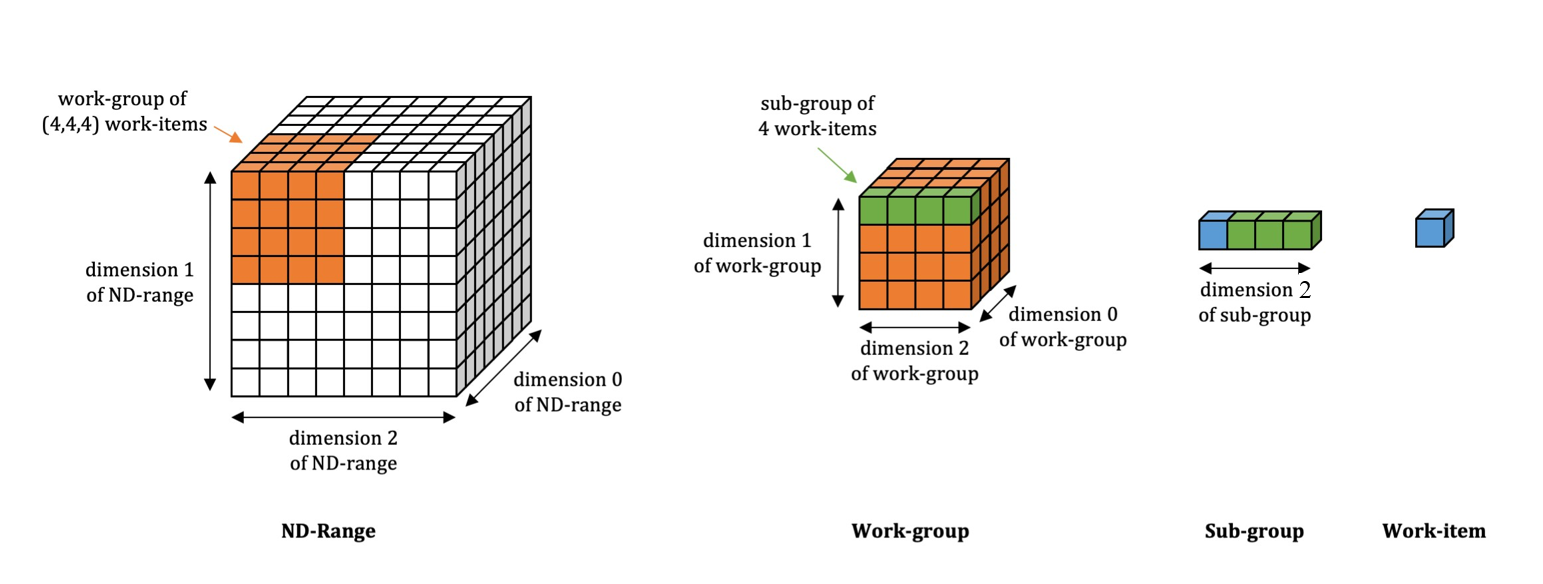
\includegraphics[width=0.9\textwidth]{2_framework/research_objective_2_sycl_eval/sycl.png}\par % Replace with your image file
\end{frame}

%% ------------------------------------------------------------------
%% SYCL Execution Model
%% -----------------------------------------------------------------

\begin{frame}{SYCL Execution Model in a Nutshell}
  \begin{columns}
    \column{0.3\textwidth}
      \tiny
      \begin{description}
        \item[Host] submits \texttt{queue.submit()} with a \texttt{kernel\_name}.
        \item[ND-Range] $\langle\,\text{global}\;3\!\times\!\text{local}\,\rangle$ defines grid.
        \item[Work-Group] maps to CUDA block / OpenCL work-group.
        \item[Sub-Group] (warp/wavefront) gives warp-level shuffle & ballot ops.
        \item[Device USM] used for persistent bit-packed buffers.
      \end{description}
    \column{0.7\textwidth}
      \centering
      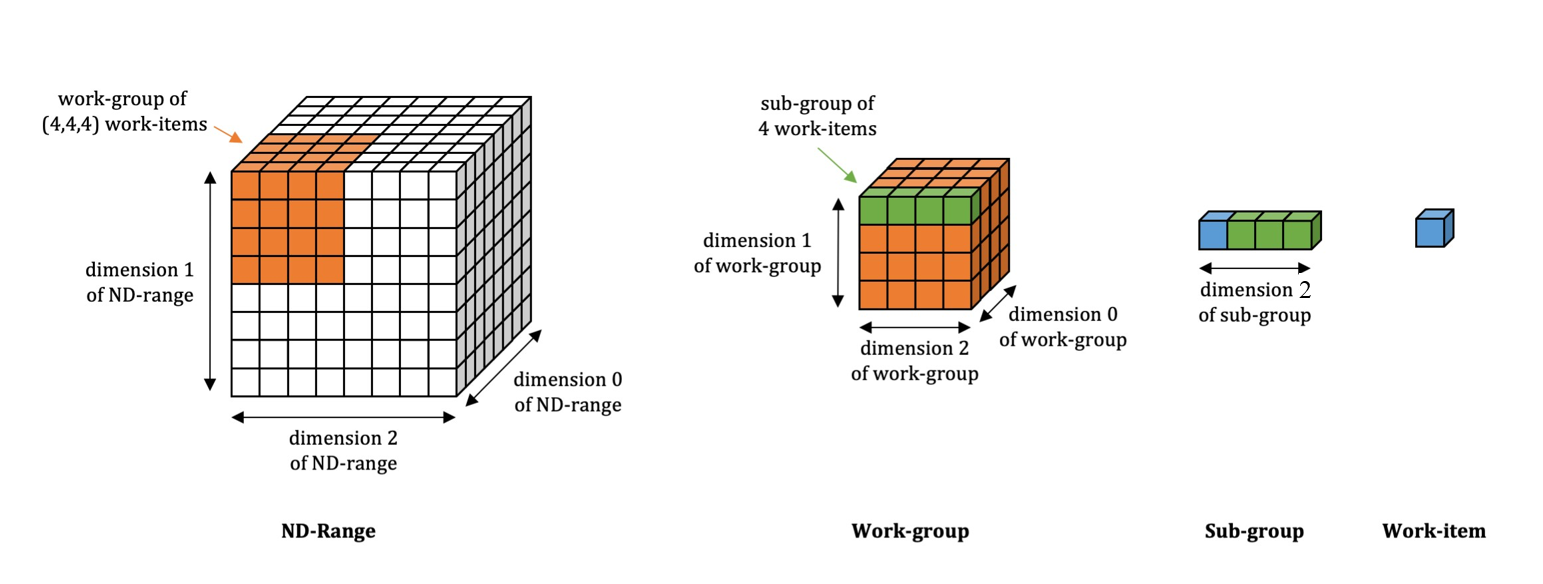
\includegraphics[width=1\textwidth]{2_framework/research_objective_2_sycl_eval/sycl.png}\par % Replace with your image file
  \end{columns}
\end{frame}

%% ------------------------------------------------------------------
%% Mapping PDAG Layers to Kernels
%% ------------------------------------------------------------------
\subsection{Kernel Execution}
\begin{frame}{Mapping PDAG Layers to SYCL Kernels}
    \tiny
  \begin{enumerate}
    \item Topological sort $\Rightarrow$ depth index $d$.
    \item All nodes with depth $d$ share \emph{identical fan-in length}.  \texttt{range<3>} := $(\text{batch},\text{gate},\text{bitpack})$.
    \item One kernel per layer; gate type dispatched via template specialization.
    \item Streams results to next-depth buffer in global memory.
  \end{enumerate}
  \vspace{-42pt}
  \begin{columns}
      \column{0.6\textwidth}
        \centering
      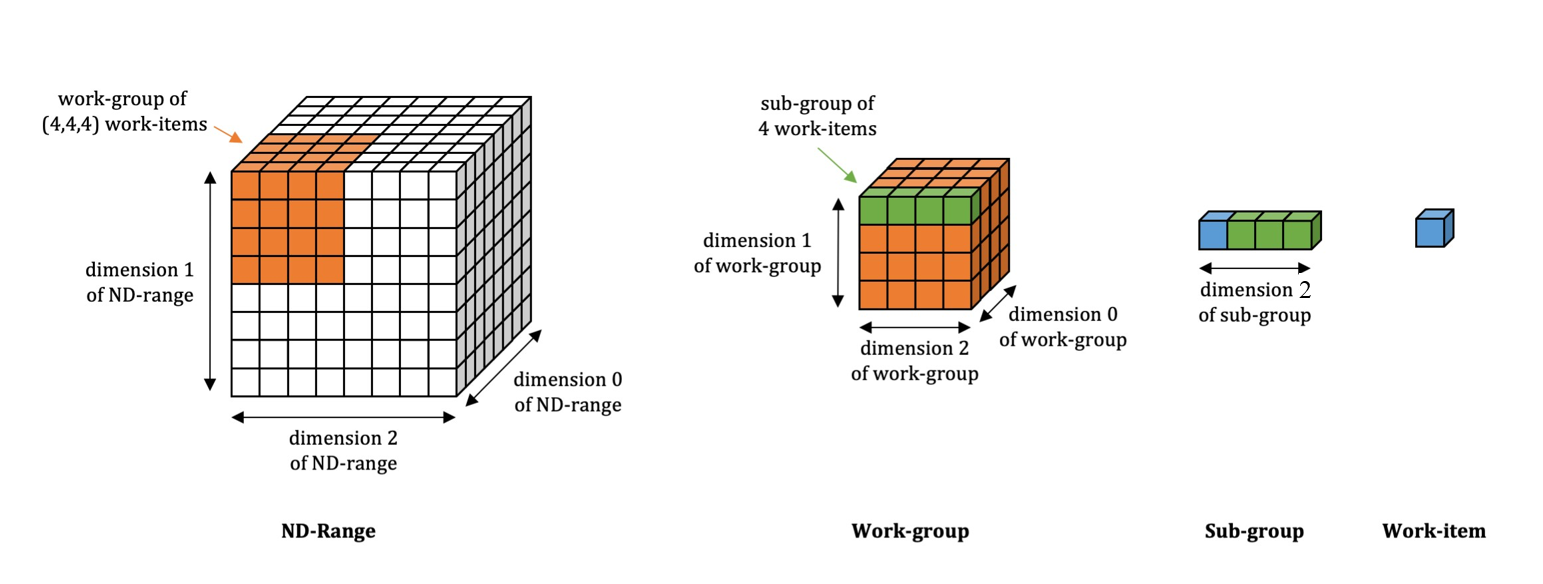
\includegraphics[width=1\textwidth]{2_framework/research_objective_2_sycl_eval/sycl.png}
      \column{0.4\textwidth}
        \centering
        \includesvg[height=0.9\textheight]{1_concepts/dag_pass_2.svg}
  \end{columns}

\end{frame}

\begin{frame}{Eval Query Performance on Generic Backends}
\centering
        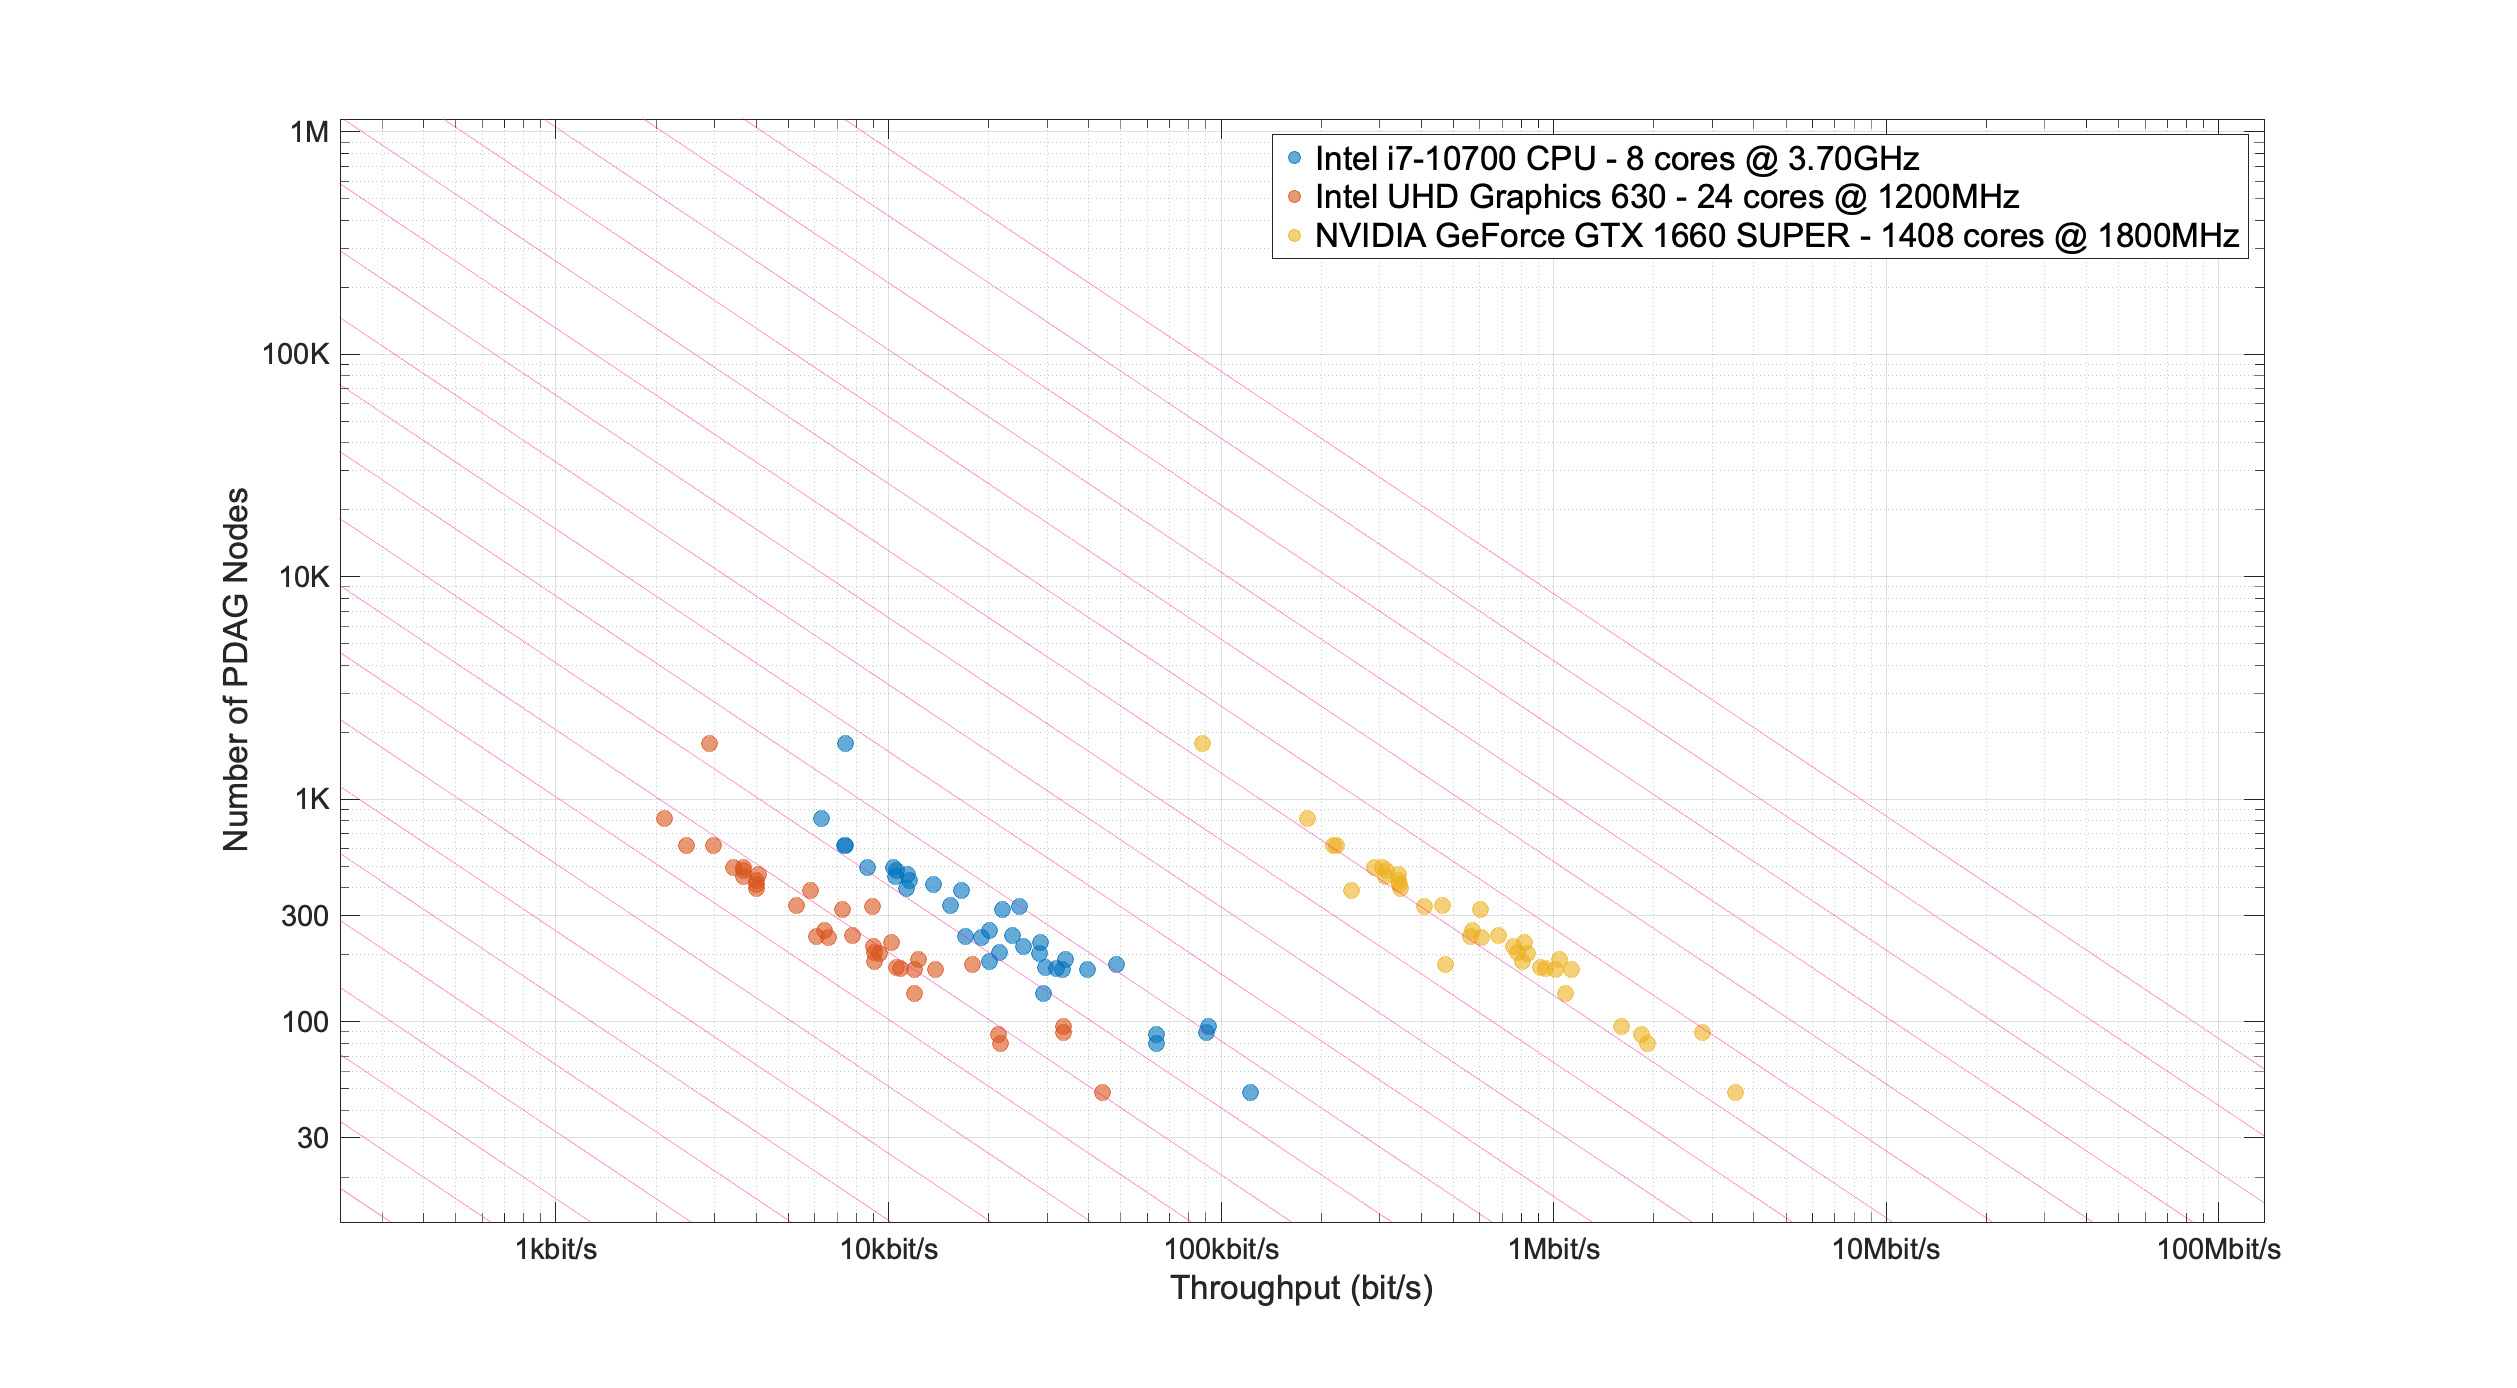
\includegraphics[height=0.9\textheight]{2_framework/research_objective_2_sycl_eval/slides_nodes_vs_throughput.eps}
\end{frame}

\begin{figure}[hb]
    \centering
    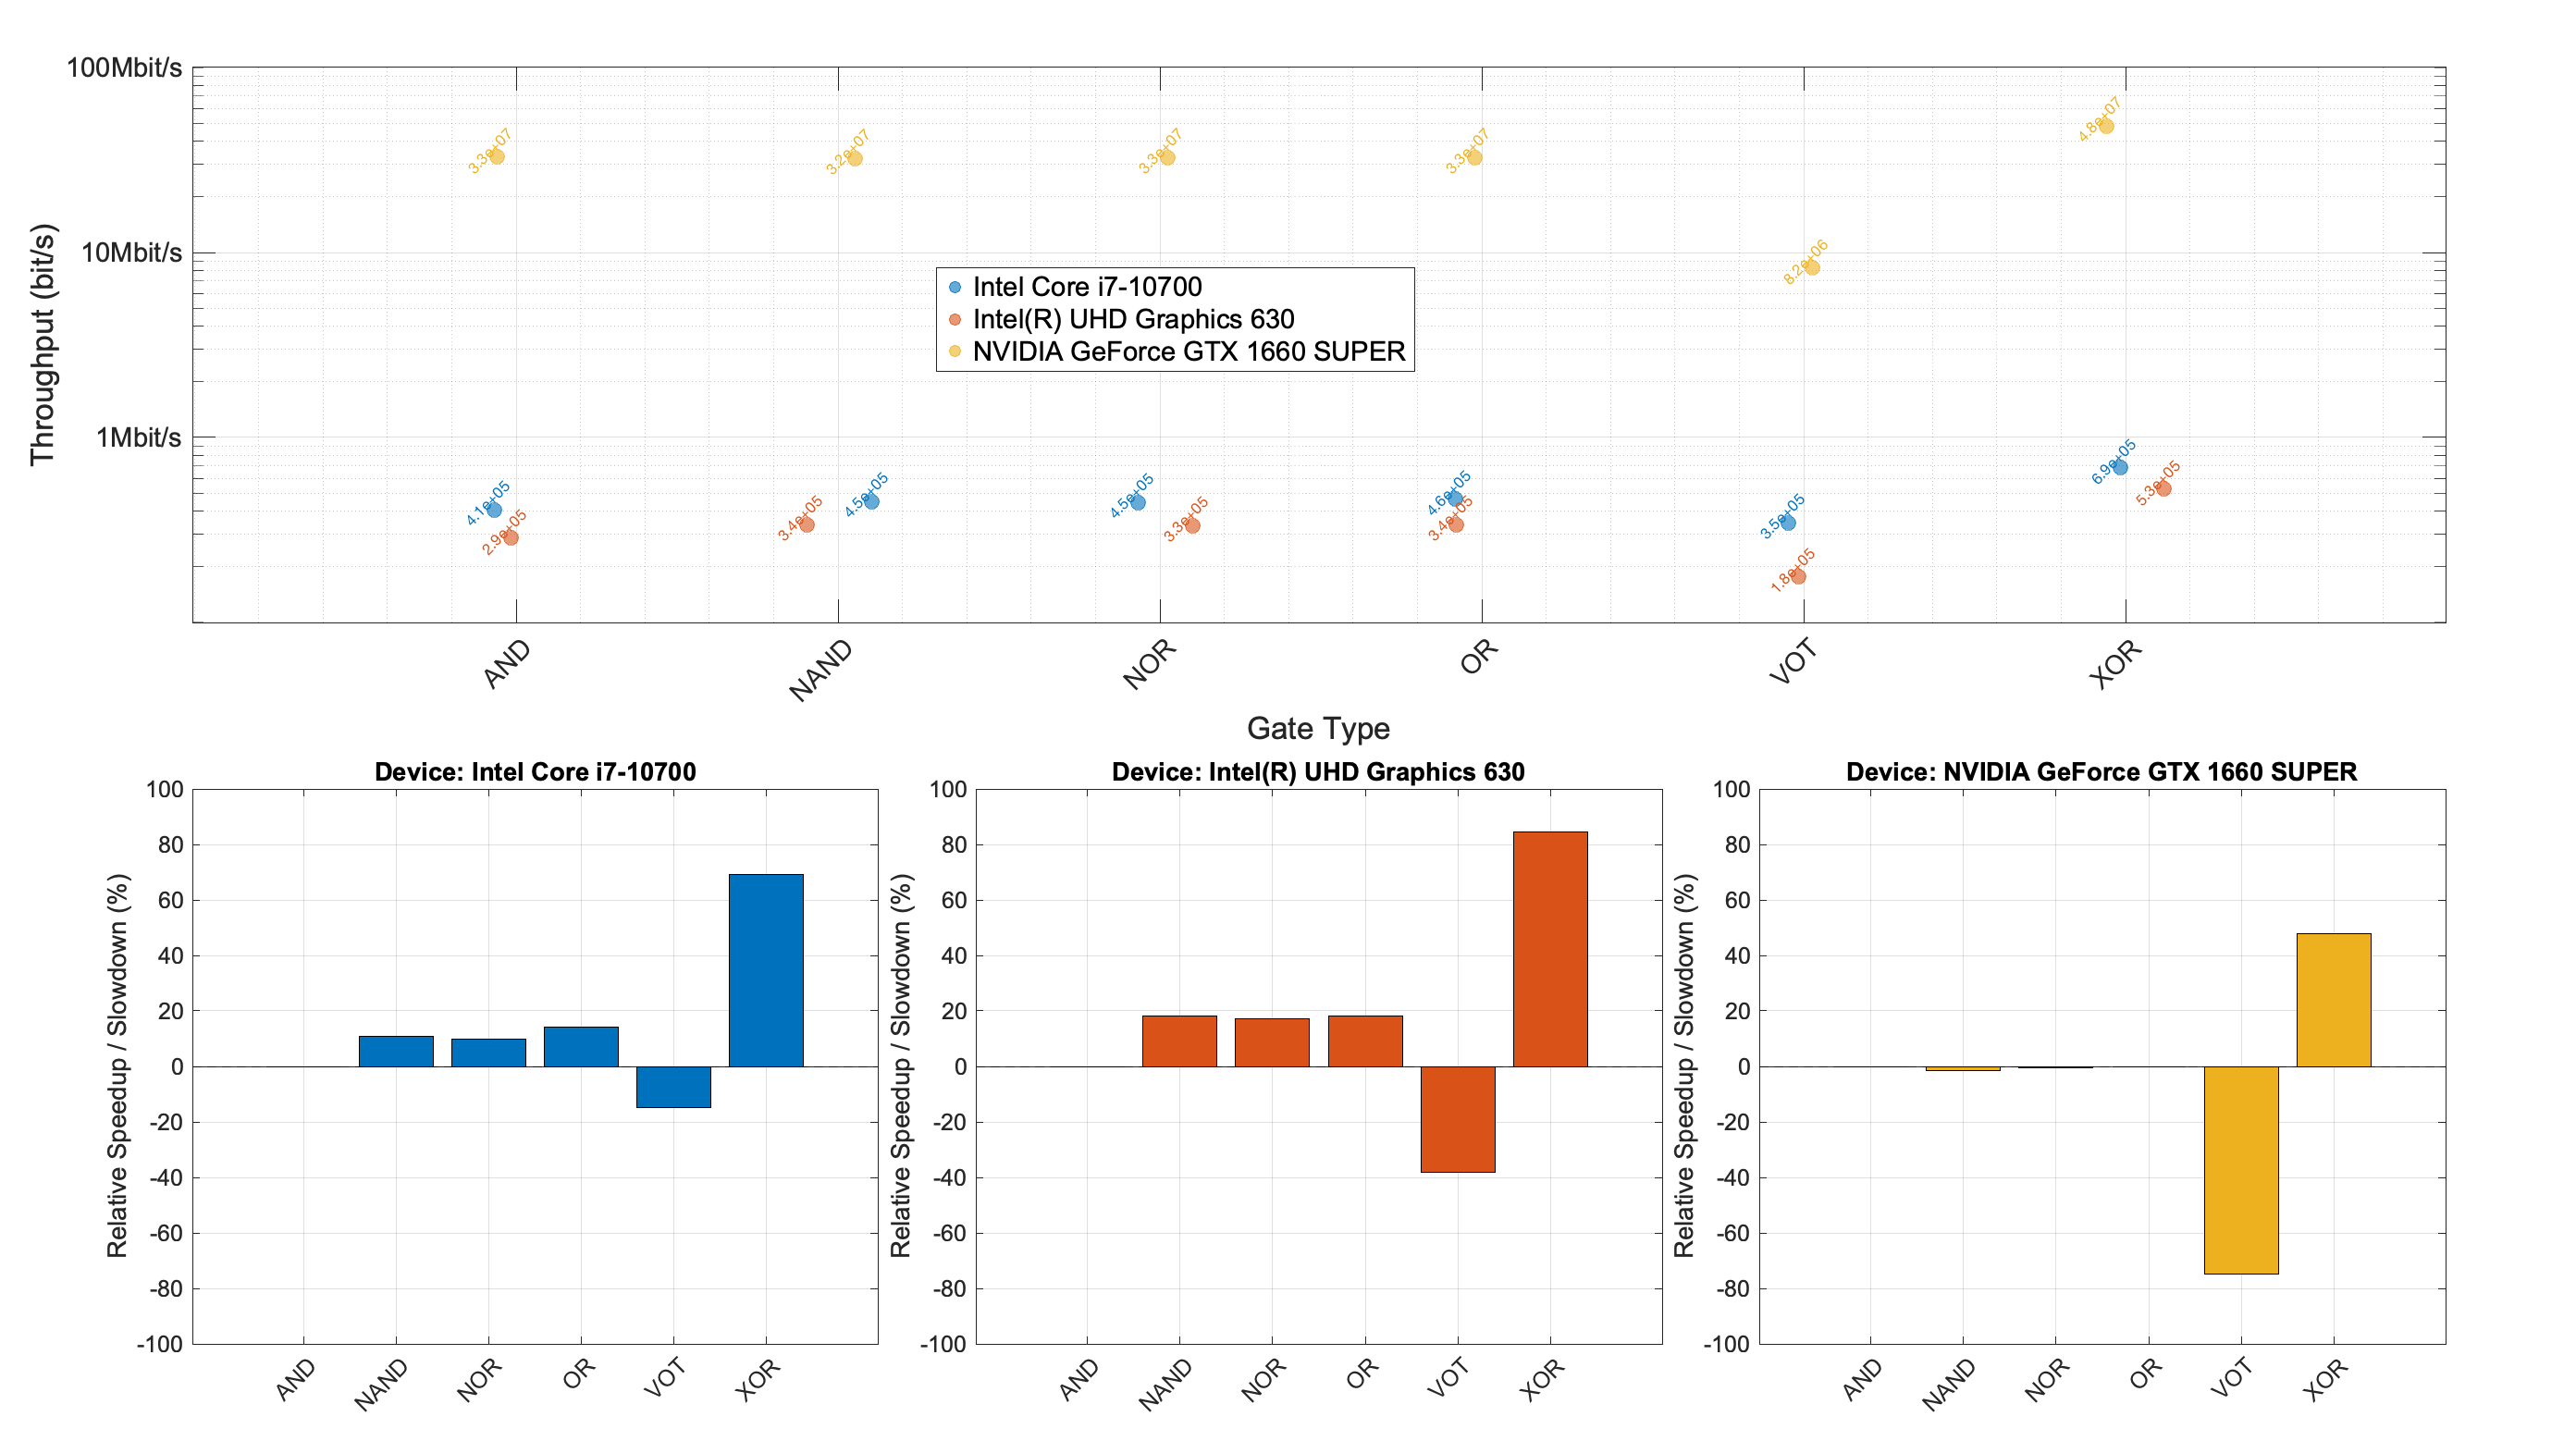
\includegraphics[height=0.8\textheight]{execution_model/slides_throughput_by_gate_type.eps}
    \caption{(Top) Throughput in bit/second on various backends for different gate types. (Bottom) \% Relative speedup/slowdown as compared to the AND gate.}
    \label{fig:gate_throughput}
\end{figure}

%% throughput graph
\begin{frame}{Eval Query Performance on Discrete GPUs}
  \begin{columns}
    \column{0.60\textwidth}
    {
      \begin{itemize}
          \item {Latency: 20-30 $ms$ per layer.}
          \item {Throughput: Graph depth and VRAM bound (see plot).}
          \item {Benchmarked on Nvidia GTX 1660 [6GB].}
          \item {Graph sizes: from $\approx 50$ to $\approx 2000$ nodes.}
          \item {Evals: from 16M to 1B per node per pass.}
      \end{itemize}
      \vspace{10pt}
      \textbf{Q: Are these enough samples to estimate the Expectation Query?}
    }
     \column{0.4\textwidth}
        \centering
        \includesvg[height=0.9\textheight]{1_concepts/mem_allocation_lines_zoom.svg}
  \end{columns}
\end{frame}





% ============================================================================
%  Research Objective 3 — Monte-Carlo Probability Estimation
%  Replaces prior preliminary version; integrates new pipeline & diagnostics
% ============================================================================
\section{Research Objective 3: Develop data-parallel Monte Carlo algorithms for probability estimation}

% ----------------------------------------------------------------------------
%  Title Frame
% ----------------------------------------------------------------------------
\begin{frame}
  \Large\centering\textbf{Research Objective 3}\\[6pt]
  \large Develop data-parallel Monte-Carlo methods for estimating probabilities on unified PDAGs
\end{frame}

% ----------------------------------------------------------------------------
%  Bridge: From Boolean Evaluation to Probabilistic Inference
% ----------------------------------------------------------------------------
\begin{frame}{Bridging Boolean Evaluation and Probabilistic Inference}
  \begin{itemize}
    \item Previous objective delivered \emph{bit-parallel gate kernels} that evaluate a PDAG layer in $\mathcal{O}(1)$ machine words.
    \item To quantify \alert{risk}, we must attach \emph{probability distributions} to the PDAG leaves and propagate forward.
    \item Strategy: embed a Monte-Carlo engine that
          \begin{enumerate}
            \item draws bit-packed Bernoulli samples for \textbf{all} basic events, and
            \item reuses the same gate kernels to evaluate each random draw.
          \end{enumerate}
    \item One kernel pipeline therefore suffices for \textbf{both} deterministic logic and stochastic sampling.
  \end{itemize}
\end{frame}

\subsection{Back to Working Example: One Initiating Event, Three Fault Trees, Six Basic Events, Five End States}
\begin{frame}
  \begin{columns}
    \column{0.66\textwidth}
      \includesvg[height=\textheight]{1_concepts/dag_pass_3.svg} % Replace with your image file
     \column{0.33\textwidth}
      \includesvg[width=\linewidth]{1_concepts/pra-model.svg} % Replace with your image file
  \end{columns}  
\end{frame}

% ----------------------------------------------------------------------------
%  End-to-End Sampling Pipeline
% ----------------------------------------------------------------------------
\begin{frame}{End-to-End Sampling Pipeline (one iteration)}
  \begin{columns}
    \column{0.6\textwidth}
      \includesvg[height=0.9\textheight]{1_concepts/dag_pass_3.svg} % Replace with your image file
     \column{0.4\textwidth}
  \tiny   
  \begin{enumerate}[<+->]
    \item \textbf{Basic-Event Kernel:} generate random draws.
    \item \textbf{Gate Kernels:} evaluate PDAG layers using hardware-native logic primitives.
    \item \textbf{Tally Kernel:} count number of ones, update counters, compute estimates.
  \end{enumerate}
  \end{columns}  
\end{frame}

% ----------------------------------------------------------------------------
%  Monte-Carlo Algorithm Recap (keeps most of prior text)
% ----------------------------------------------------------------------------
\subsection{MC Sampling Theory}

\begin{frame}{Monte-Carlo Sampling over PDAGs}
  \small
  \begin{enumerate}
    \item Draw $\mathbf{x}^{(i)}\sim\prod_{b\in\mathcal{B}}\text{Bernoulli}\bigl(p_b\bigr)$ in \textbf{bit-packed} form.
    \item Evaluate the Boolean function $F\colon\{0,1\}^{|\mathcal{B}|}\!\to\!\{0,1\}$ (root node) using the gate kernels.
    \item Record $Y^{(i)} \!=\! F\bigl(\mathbf{x}^{(i)}\bigr)$ \;(failure indicator).
  \end{enumerate}
  After $N$ iterations
  \[\widehat{P}_N = \frac1N\sum_{i=1}^N Y^{(i)},\qquad \operatorname{SE}(\widehat P_N)=\sqrt{\frac{\widehat P_N(1-\widehat P_N)}{N}}.\]
  Error shrinks as $\mathcal{O}\!\bigl(N^{-1/2}\bigr)$; variance-reduction extensions discussed shortly.
\end{frame}


% ----------------------------------------------------------------------------
%  Basic-Event Sampling Kernel
% ----------------------------------------------------------------------------
\begin{frame}{Basic-Event Sampling Kernel}
\begin{columns}
  \column{0.7\textwidth}
  \footnotesize
  \begin{itemize}
    \item Each basic event $b\in\mathcal{B}$ is modelled as an independent \textbf{Bernoulli} random variable $X_b\sim\operatorname{Bernoulli}(p_b)$.
    \item A single Monte--Carlo iteration packs $\omega = 8\,\mathrm{sizeof}(\texttt{bitpack\_t}) = 64$ independent trials into one machine word.
    \item For batch index $b$, bit--pack $p$, lane $\lambda$:
          $\displaystyle X_{b,p,\lambda}\sim\operatorname{Bernoulli}(p_b)$.
    \item The basic--event kernel uses the counter--based \textsc{Philox--4×32--10} PRNG; counters are derived from $(b,p,\lambda,t)$, guaranteeing reproducibility and inter--thread independence.
    \item After one iteration ($N = B P \omega$ trials) the sufficient statistics per basic event are
          $\displaystyle s_b = \sum_{p,\lambda} X_{b,p,\lambda}$,\;
          $\widehat p_b = s_b/N$,\;
          $\operatorname{SE}(\widehat p_b)=\sqrt{\widehat p_b(1-\widehat p_b)/N}$.
  \end{itemize}
       \column{0.3\textwidth}
       \includesvg[width=\textwidth]{2_framework/research_objective_3_mc_sampling/sample_event_A.svg}\par
  \end{columns}
\end{frame}


%% needs a frame on tallies, with estimator statistics, convergence properties
% ----------------------------------------------------------------------------
%  Tally Kernel & Estimator Convergence
% ----------------------------------------------------------------------------
\begin{frame}{Tally Kernel}
  \footnotesize
  \begin{itemize}
    \item For a designated node $v$ (e.g. system top event) define $Y_{p,\lambda}^{(t)} = F_v\bigl(\mathbf{X}_{\cdot,p,\lambda}^{(t)}\bigr)\in\{0,1\}$.
    \item \textbf{Tally kernel} executes a single SIMD \texttt{popcount} per bit-pack to obtain the per-iteration count
      $\displaystyle s_v^{(t)} = \sum_{p,\lambda} Y_{p,\lambda}^{(t)}$.
    \item Cumulative statistics after $T$ iterations ($N_T = T N$ trials):
      \[ S_v = \sum_{t=1}^{T} s_v^{(t)},\qquad \widehat P_v = \frac{S_v}{N_T}. \]
    \item Unbiased variance estimator
      \[ \widehat{\sigma}^2_v = \frac{\widehat P_v\bigl(1-\widehat P_v\bigr)}{N_T}. \]
    \item \textbf{Central Limit Theorem.}  As $T\to\infty$
      \[ \frac{\widehat P_v - P_v}{\widehat \sigma_v}\;\xrightarrow{\,\mathcal{D}\,}\;\mathcal N(0,1). \]
  \end{itemize}
\end{frame}

%% run with runaway iterations.
%% show a run with too many iterations, and make the case for developing a robust convergence criteria.
% ----------------------------------------------------------------------------
%  The Cost of Runaway Iterations (Motivation)
% ----------------------------------------------------------------------------
\begin{frame}{When "More Samples" is Wasteful}
  \begin{columns}
    \column{0.35\textwidth}
      \footnotesize
      \begin{itemize}
        \item Fixed iteration budgets ($N$ large and hard-wired) risk \emph{massive}\, oversampling when $P_v$ is moderate (\(\approx10^{-4}\)–\(10^{-1}\)).
      \end{itemize}
    \column{0.65\textwidth}
      \centering
      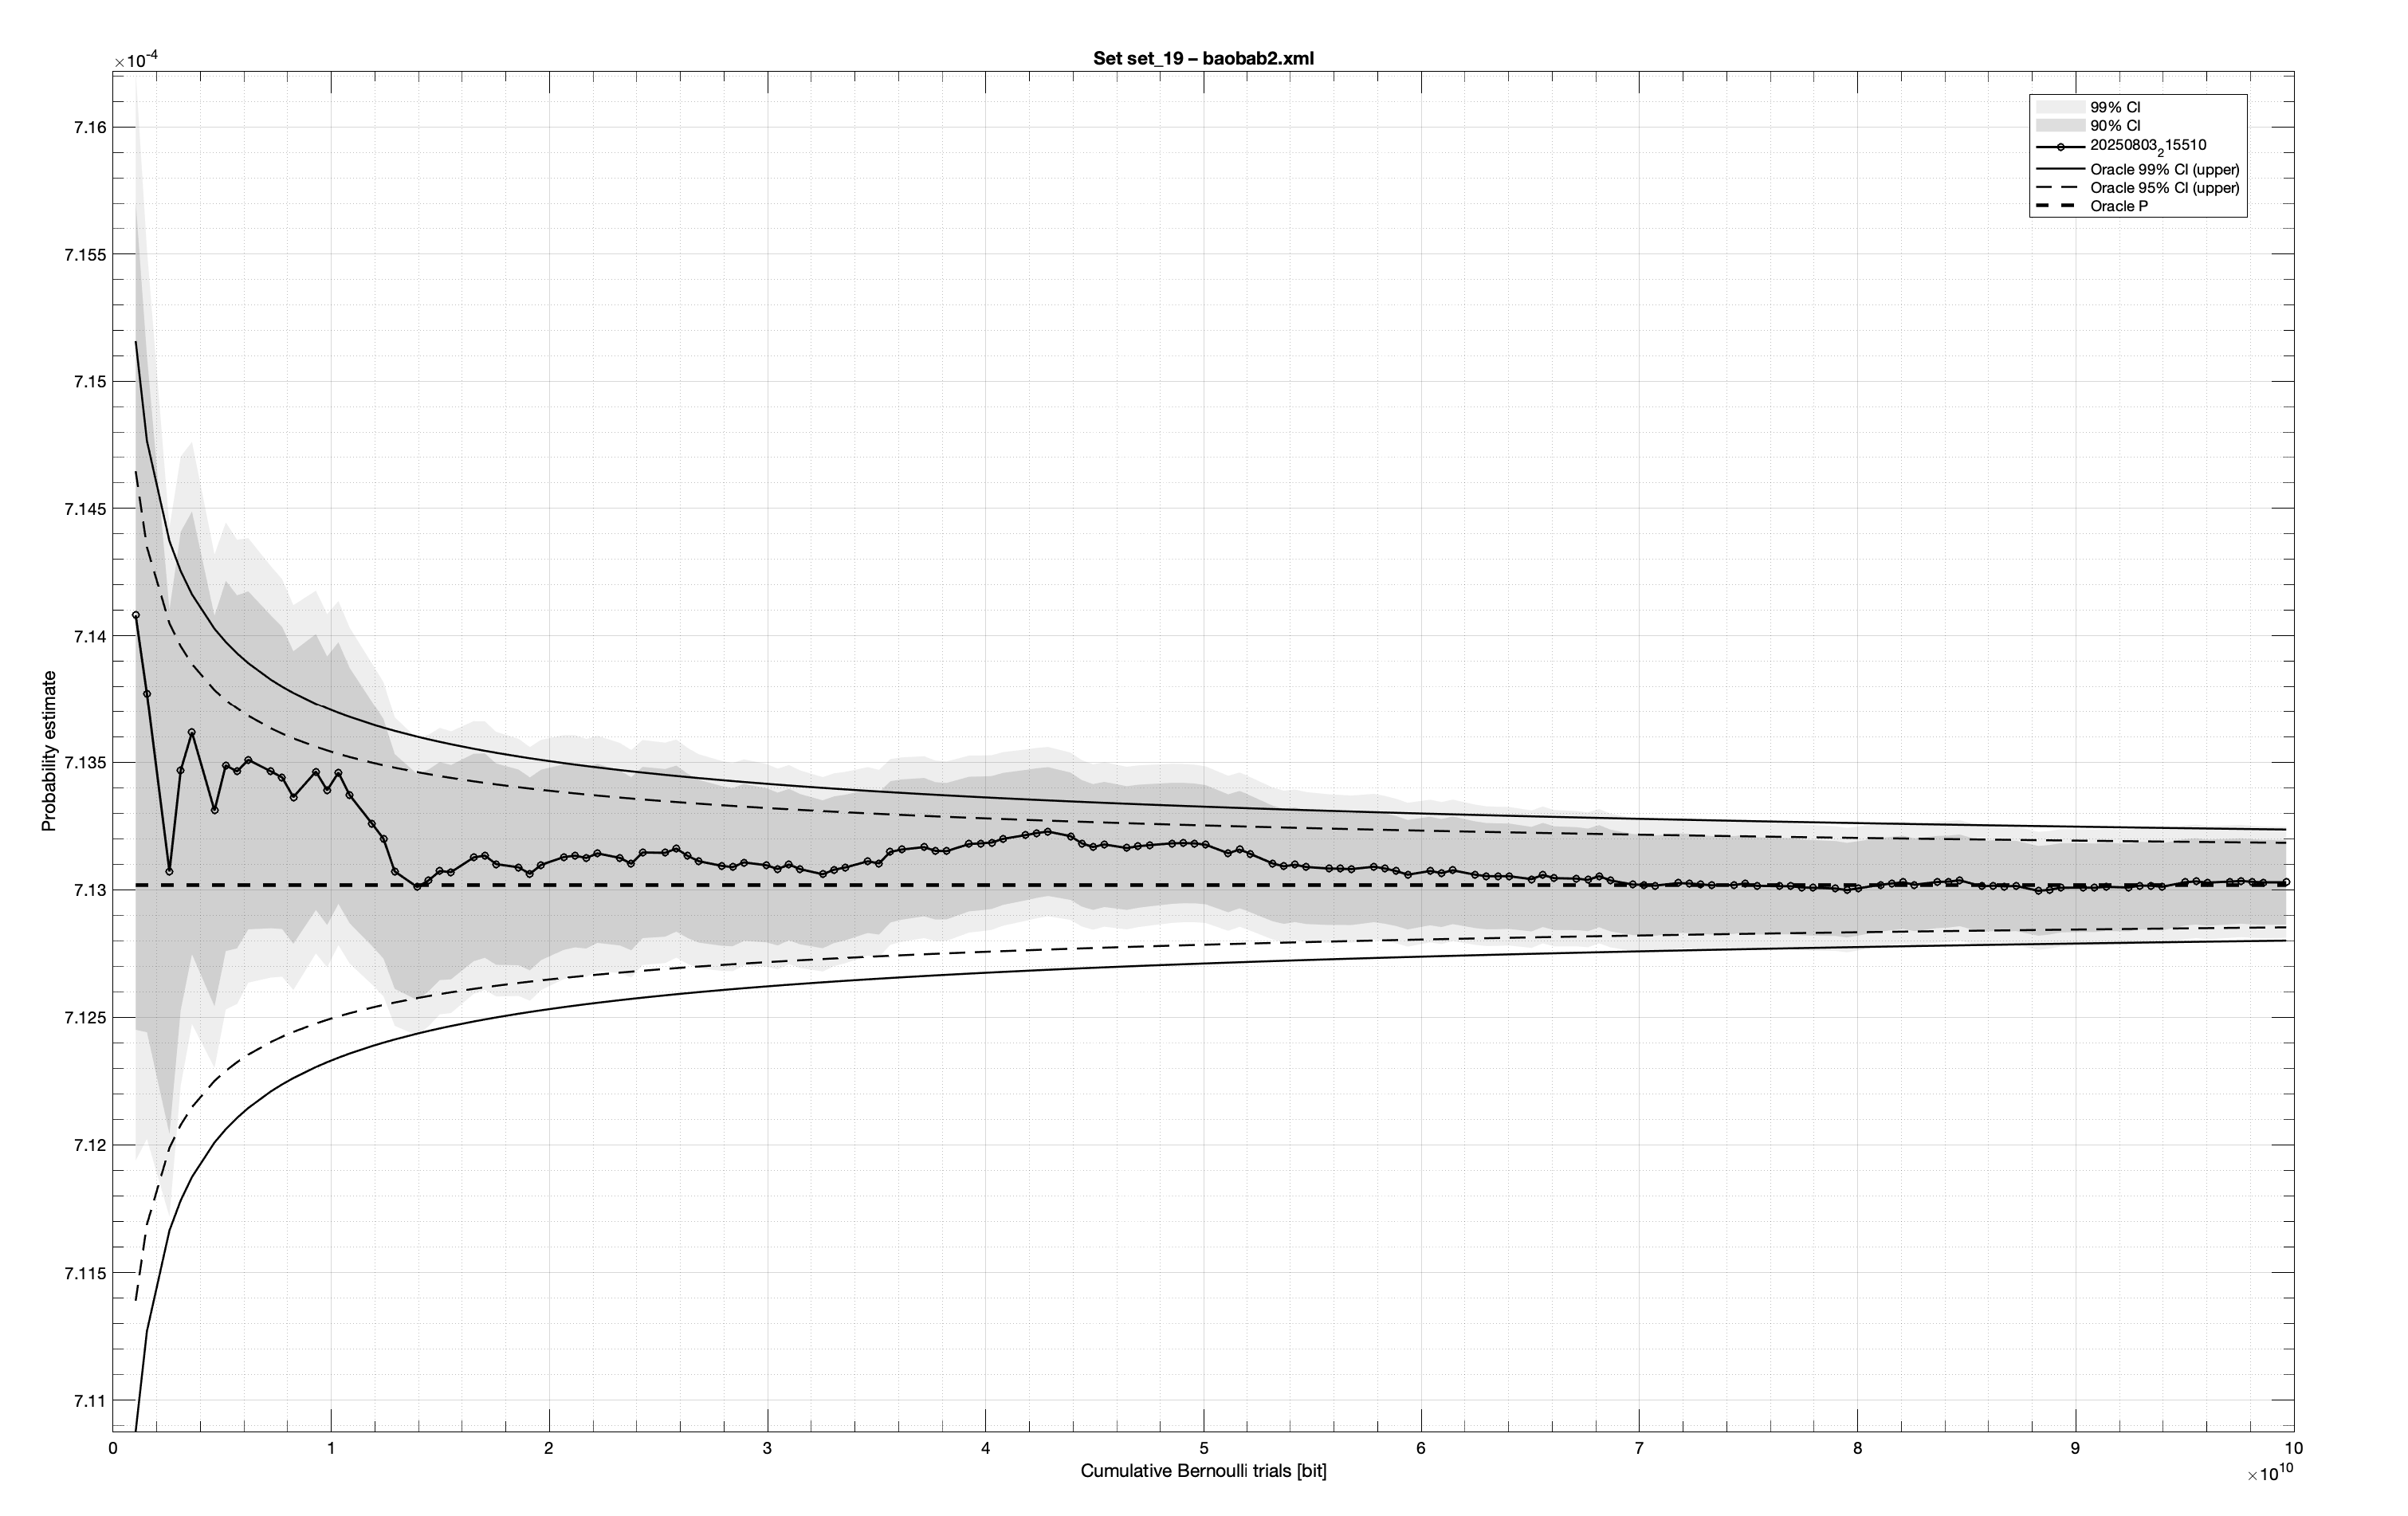
\includegraphics[width=0.95\linewidth]{2_framework/research_objective_3_mc_sampling/conv_fig_02.eps} % create trace: half-width vs iterations
      \vspace{-6pt}
  \end{columns}
\end{frame}

\subsection{Building a Monte Carlo Estimator for Event Probabilities}
\begin{frame}[t, allowframebreaks]
\frametitle{Boolean Functions: Basic Concepts}
\begin{itemize}
  \item Let \(\mathbf{x} = (x_1, x_2, \dots, x_n)\) be a vector of \(n\) Boolean variables, each \(x_i \in \{0,1\}\).
  \item A \emph{Boolean function} is any map \(F(\mathbf{x}): \{0,1\}^n \to \{0,1\}\).
  \item Example: If \(F\) encodes “system fails,” then \(F(\mathbf{x}) = 1\) signifies a failure mode, where \(\mathbf{x}\) captures component states.
  \item Modeling perspective:
    \begin{itemize}
      \item AND, OR, NOT, \(k\)-of-\(n\) gates allow composing complex logic.  
      \item Each \(F\) can be evaluated deterministically if we know \(\mathbf{x}\).
    \end{itemize}
\end{itemize}
\end{frame}

\begin{frame}[t, allowframebreaks]
\frametitle{Exact Probability Estimation: Inclusion-Exclusion}
\begin{itemize}
  \item Suppose each \(x_i\) has a probability \(p_i = \Pr[x_i=1]\), assuming independence.
  \item We want \(\Pr[F(\mathbf{x}) = 1]\), which is
  \[
    \Pr\bigl[F(\mathbf{X})=1\bigr]
    \;=\; 
    \sum_{\mathbf{x}\in \{0,1\}^n}
      F(\mathbf{x}) 
      \prod_{i=1}^n
      \bigl[p_i^{\,x_i}(1-p_i)^{\,1-x_i}\bigr].
  \]
  \item For sets of events, using the \emph{inclusion-exclusion principle}:
  \[
    \Pr\Bigl(\bigcup_{i=1}^n E_i\Bigr)
    \;=\;
    \sum_{k=1}^n \;(-1)^{k+1} 
    \;\;\sum_{1\le i_1< \cdots < i_k\le n}
    \!\Pr\bigl(E_{i_1}\cap\dots\cap E_{i_k}\bigr).
  \]

\end{itemize}
\end{frame}

\begin{frame}[allowframebreaks]
\frametitle{Approximation Methods: REA and MCUB}
 For large \(n\), exact enumeration of subsets is exponential, making it impractical for large Boolean circuits.
 \vspace{8pt}
\begin{itemize}
  \item \textbf{Rare-Event Approximation (REA):}
    \begin{itemize}
      \item Assumes each event has small probability \(p_i \ll 1\).
      \item Overlaps (intersections of multiple failures) are deemed negligible.
      \item Probability of the union \(\approx \sum_{i} \Pr[E_i]\), ignoring higher-order terms.
    \end{itemize}
\framebreak
  \item \textbf{Min-Cut Upper Bound (MCUB):}
    \begin{equation}
    \label{eq:mcub_slides}
      \Pr\Bigl[\bigcup_{C \in \{\mathrm{MCS}\}} C\Bigr]
      \;\le\;
      \sum_{C \in \{\mathrm{MCS}\}}
      \;\prod_{b \in C} p_b ,
    \end{equation}
    \begin{itemize}
      \item Interprets each minimal cut set (MCS) as a distinct mechanism for failure.
      \item Sums (over)estimate total failure if MCSs share components.
      \item Often used as a conservative bound in safety analyses.
    \end{itemize}
  \vspace{6pt}
  \item Both methods reduce complexity but can misestimate the true probability when events are not truly rare or heavily intersect.
\end{itemize}
\end{frame}



\begin{frame}[t]
\frametitle{Boolean Derivatives: Definition and Interpretation}
\begin{itemize}
\item \textbf{Boolean Derivative Concept:}  
  For a Boolean function \(F(\mathbf{x})\) with \(\mathbf{x}=(x_1,\ldots,x_n)\), the derivative with respect to \(x_i\) is defined via XOR:
  \[
    \frac{\partial F}{\partial x_i}
    \;=\;
    F(x_i=0,\mathbf{x}_{-i})
    \;\oplus\;
    F(x_i=1,\mathbf{x}_{-i}),
  \]
  where \(\oplus\) denotes the exclusive-OR operation, and \(\mathbf{x}_{-i}\) are all variables except \(x_i\).
\item \textbf{Interpretation:}  
  \begin{itemize}
    \item \(\frac{\partial F}{\partial x_i}(\mathbf{x})=1\) whenever \emph{flipping} \(x_i\) changes the value of \(F\) under the specific configuration \(\mathbf{x}_{-i}\).  
    \item Captures \emph{sensitivity}: if \(\frac{\partial F}{\partial x_i}\) rarely equals \(1\), then \(F\) is robust to changes in \(x_i\).  
  \end{itemize}
\end{itemize}
\end{frame}

\begin{frame}[allowframebreaks]
\frametitle{Extension to Monte Carlo Estimation of Boolean Derivatives}
\begin{itemize}
  \item \textbf{Key Idea:} Estimate \(\mathbb{E}[\,\partial F / \partial x_i\,]\) by sampling random configurations \(\mathbf{x}^{(s)}\) of the Boolean inputs, then checking how \(F\) changes when \(x_i\) is flipped.
  \vspace{8pt}
  \item \textbf{Sampling Procedure:}
    \begin{enumerate}
      \item Draw \(\mathbf{x}^{(s)} = \bigl(x_1^{(s)},\dots,x_n^{(s)}\bigr)\) from the distribution of interest.  
      \item Form \(\mathbf{x}^{(s)} \oplus \mathbf{e}_i\) by flipping the \(i\)th coordinate.
      \item Compute:
        \[
          \frac{\partial F}{\partial x_i}\bigl(\mathbf{x}^{(s)}\bigr)
          \;=\;
          F\!\bigl(\mathbf{x}^{(s)}\bigr)
          \;\oplus\;
          F\!\bigl(\mathbf{x}^{(s)} \oplus \mathbf{e}_i\bigr).
        \]
    \end{enumerate}
  \item \textbf{Insight:}  
    \begin{itemize}
    \item{Sensitivity and importance analysis using sampling methods.}
    \item{Gradient computation opens a path towards learning-based tasks.}
    \end{itemize}
\end{itemize}
\end{frame}

\begin{frame}[t, allowframebreaks]
\frametitle{Avoiding Inclusion-Exclusion via Monte Carlo}
\begin{itemize}
  \item Exact expansions for large circuits require enumerating all subsets of failing components or gates, which is computationally huge.
  \item In contrast, \emph{Monte Carlo} draws a sample \(\mathbf{x}\in \{0,1\}^n\) and directly evaluates \(F(\mathbf{x})\) without enumerating \emph{all} subsets.
  \item Each run picks a single draw of failed components from the distribution. After many runs, the frequency of \(F=1\) approximates its probability.
  \item Results:
    \begin{itemize}
      \item No exponential blow-up in the number of terms.
      \item Straightforward extension to complex gate structures, correlated variables.
      \item Parallelizable on modern CPU/GPU architectures.
    \end{itemize}
\end{itemize}
\end{frame}

\begin{frame}[t, allowframebreaks]
\frametitle{Data-Parallel Implementation using SYCL}
\item \textbf{Data-Parallel Monte Carlo for Boolean Circuits:}
  \begin{itemize}
    \item{Simultaneous evaluation of \emph{all} intermediate gates, success, and failure paths.}
    \item{Relax coherence constraints - arbitrary shapes with NOT gates permitted.}
    \item{Vectorized bitwise hardware ops for logical primitives (AND, OR, XOR, etc.)}
    \item{Specialized treatment of \(k/n\) logic, without expansion.}
    \item{Simultaneous use of all available compute - GPUs, multicore CPUs.}
    \vspace{16pt}
  \end{itemize}
\end{frame}